% compendium/energy-commodities/futures-hedging.tex
% Entries migrated on 2026-10-15 from the legacy Hull notes (slice 31, volatility-options/fwdfut.tex), owned by
% commodity-hedging, one of the file's map candidates. Dispositions in notes/migration-slices.md; the file verbatim in
% notes/artefacts/volatility-options/.

\section{Hedging with futures}

\begin{qfdefinition}[Futures hedges and basis: short and long hedges, the basis, basis risk, cross hedging, contract choice and stack and roll]\label{def:futures-hedge-basis}
\qffield{Statement} Hull treats \emph{hedge-and-forget} strategies: a futures position is taken at the start and closed at the end, with no adjustment in between \citep[chap.~3, ``Hedging Strategies Using Futures'', p.~70]{s7-hulloptions}. A \emph{short hedge}, a short futures position, suits a hedger who owns or will own an asset and expects to sell it; a \emph{long hedge} suits one who will buy an asset and wants to lock in a price now (sec.~3.1, pp.~71--72). The \emph{basis} is ``spot price of asset to be hedged $-$ futures price of contract used''; an increase is a strengthening, a decrease a weakening (sec.~3.3, p.~76). With spot $S_i$, futures $F_i$ and basis $b_i=S_i-F_i$ at the start $t_1$ and end $t_2$, the effective price obtained or paid with a hedge is
\[ S_2+F_1-F_2=F_1+b_2 \]
for both short and long hedges (p.~77); $F_1$ is known at $t_1$, and the uncertainty in $b_2$ is \emph{basis risk}. \emph{Cross hedging} uses a futures contract on a different asset (p.~77; sec.~3.4, p.~79); with $S_2^*$ the price at $t_2$ of the asset underlying the futures, Hull writes the hedged price $S_2+F_1-F_2$ as
\[ F_1+(S_2^*-F_2)+(S_2-S_2^*), \]
whose two last terms are ``the two components of the basis'': $S_2^*-F_2$ is the basis that would exist if the hedged asset were the futures' underlying (the futures-underlying basis), and $S_2-S_2^*$ is ``the basis arising from the difference between the two assets'' (p.~77). Both expressions assume a hedge ratio of 1.0, one futures unit per unit of exposure, which Hull calls natural when the two assets are the same and ``not always optimal'' in a cross hedge (p.~79). Interpretation, derived here: with a hedge ratio $h$, the size of the futures position per unit of exposure taken in the direction that offsets it (short for a seller, long for a buyer), the effective price received or paid per unit is
\[ S_2+h(F_1-F_2), \]
which reduces to $F_1+b_2$ at $h=1$; $h=0$ is no hedge and a negative $h$ would add to the exposure. Prices are per unit of each asset, and $h$ is in futures units per unit of exposure, so it carries any conversion between the two assets' units (none is needed in Hull's jet-fuel and heating-oil example, both in gallons).

\qffield{Conditions} Hedges are imperfect because the hedged asset may differ from the futures' asset, the date of purchase or sale may be uncertain, and the futures may have to be closed before its delivery month (pp.~75--76). Basis changes can help or hurt: an unexpected strengthening improves a short hedger's position and worsens a long hedger's (p.~77). Hull defines the basis as spot minus futures but notes the reverse definition is sometimes used, especially for financial futures (p.~76, n.~2); the sign convention must be stated. As a rule of thumb, Hull chooses the delivery month closest to, but after, the hedge's end, because basis risk grows with the gap and prices can be erratic in the delivery month; the rule assumes enough liquidity (p.~78). When the hedge outlasts all liquid contracts, \emph{stack and roll} closes one contract and opens a later one, repeatedly; Metallgesellschaft's rolled hedges in the early 1990s produced cash outflows before the offsetting gains on its supply contracts, a liquidity problem (sec.~3.6, pp.~89--90).

\qffield{Practice} Checked with Hull's examples: an oil producer shorting August futures at \$49 against a spot of \$50 realises about \$49 a barrel whether spot ends at \$45 (a \$4 futures gain) or \$55 (a \$6 loss) (p.~71); $S_1,F_1,S_2,F_2=2.50,2.20,2.00,1.90$ give $b_1=0.30$, $b_2=0.10$ and an effective price of 2.30 (p.~77); the yen hedge gives $1.0800+(-0.0050)=1.0750$ cents and \$537{,}500 for 50 million yen (Example~3.1, pp.~78--79); the oil purchase gives $48.00+0.90=48.90$ and \$978{,}000 (Example~3.2, p.~79); the rolled oil hedge earns $0.80+0.50+0.40=1.70$ a barrel against a \$3 fall in spot (p.~90).

\qffield{Pitfalls} The legacy table added a long-hedge column beside Hull's short-hedge oil example, with a loss of 4 and a gain of 6; Hull's oil example is a short hedge only, and his long-hedge example is copper (pp.~71--72). The mirror-image column is arithmetically consistent (a buyer paying the August spot and losing or gaining on a long hedge also ends near \$49) but is not Hull's. The legacy's three causes of imperfection are Hull's (pp.~75--76). Whether hedging adds value to a firm, and time-varying hedge ratios, are outside these passages (backlog).

\qffield{See also} \hyperref[mod:minimum-variance-hedge-ratio]{minimum-variance hedge ratio}; \hyperref[def:derivative-contracts]{derivative contracts} (convergence); \hyperref[res:cost-of-carry-forward-price]{cost-of-carry forward price} (why futures and spot differ before delivery); \hyperref[def:arbitrage]{arbitrage} (Harris's basis).

\qffield{Further reading} The pathway's readings on why firms hedge and on dynamic hedge ratios are named in its backlog. The legacy file is kept verbatim in \nolinkurl{notes/artefacts/volatility-options/}.

\qffield{Index} hedge-and-forget; short hedge; long hedge; basis; strengthening of the basis; weakening of the basis; basis risk; effective price; cross hedging; choice of delivery month; stack and roll; rolling hedges; Metallgesellschaft

\qffield{Status} Verification: partly checked 2026-10-15 (against the text layer of a local copy of \texttt{s7-hulloptions}, 11th Global edition, chap.~3, pp.~70--79 and 89--90, printed page $=$ PDF page $-1$; five examples recomputed; the basis components and hedge-ratio wording rechecked 2026-10-16, pp.~77--79; the general-$h$ expression derived here). Stability: draft. Currency: concepts timeless; contract examples as of 2021.
\end{qfdefinition}

\begin{qfmodel}[Minimum-variance hedge ratio: derivation, hedge effectiveness, number of contracts, daily settlement and tailing, and beta hedges with index futures]\label{mod:minimum-variance-hedge-ratio}
\qffield{Statement} The \emph{hedge ratio} is the size of the futures position over the size of the exposure \citep[chap.~3, ``Hedging Strategies Using Futures'', sec.~3.4, p.~79]{s7-hulloptions}. Ignoring daily settlement, with $\Delta S$ and $\Delta F$ the changes in spot and futures prices over the life of the hedge and $\Delta S=a+b\,\Delta F+\epsilon$ approximately linear, a hedger long the asset and short $h$ futures per unit holds $\Delta S-h\Delta F=a+(b-h)\Delta F+\epsilon$, whose variance is minimised at $h=b$ (p.~80):
\[ h^*=\rho\,\frac{\sigma_S}{\sigma_F},\qquad N^*=\frac{h^*Q_A}{Q_F}, \]
with $\sigma_S,\sigma_F$ the standard deviations of $\Delta S,\Delta F$, $\rho$ their correlation, $Q_A$ the units hedged and $Q_F$ the units per contract (eqs.~(3.1)--(3.2), pp.~80--81). Hedge effectiveness, the share of variance removed, is the regression $R^2$, equal to $\rho^2$ (p.~81).

\qffield{Notation} $\Delta S,\Delta F$ price changes per unit, in the same price units; $h$ dimensionless; $N^*$ contracts. Interpretation, derived here: for a hedged position $V(h)=\Delta S-h\Delta F$, $\operatorname{Var}V(h)=\sigma_S^2-2h\rho\sigma_S\sigma_F+h^2\sigma_F^2$, a convex quadratic minimised where $d\operatorname{Var}V(h)/dh=0$, at $h^*=\rho\sigma_S/\sigma_F=\operatorname{Cov}(\Delta S,\Delta F)/\operatorname{Var}\Delta F$, the OLS slope; the minimum is $\sigma_S^2(1-\rho^2)$. A short futures position is $h>0$ against a long exposure; a hedger short the asset buys $h^*$.

\qffield{Conditions} The estimate assumes the future resembles the past; $\rho,\sigma_S,\sigma_F$ are usually estimated from equal non-overlapping intervals, ideally as long as the hedge (p.~81). The $R^2=\rho^2$ result is in-sample: it describes the estimation period and assumes the linear relation and its parameters hold over the hedge. \emph{Daily settlement.} Futures make a series of one-day hedges; with $\hat\sigma_S,\hat\sigma_F,\hat\rho$ for percentage one-day changes, the hedge from a regression of percentage changes is $\hat h=\hat\rho\hat\sigma_S/\hat\sigma_F$ and $N^*=\hat hV_A/V_F$, with $V_A=SQ_A$ and $V_F=FQ_F$; equivalently the one-day price-change hedge is $\hat\rho\hat\sigma_SS/(\hat\sigma_FF)$ (eq.~(3.3), p.~83). Price-change and return regressions therefore differ by the ratio $S/F$ and must not be mixed. \emph{Tailing}: allowing for interest on daily settlement, Hull divides $N^*$ by 1.05 for a hedge with one year left at 5 percent (p.~83); interpretation: the general factor is the growth of \$1 over the remaining life at the relevant rate, which equals $1+0.01r$ only for one year at simple rate $r$ percent.

\qffield{Practice} \emph{Checked}, recomputing Hull's Example~3.3 from his Table~3.2 data: $\sigma_F=0.0313$, $\sigma_S=0.0263$, $\rho=0.928$, $h^*=0.778$ and $N^*=0.778\times2{,}000{,}000/42{,}000=37.0$, so 37 contracts (p.~82). The same $h^*$ results from minimising the sample variance of $\Delta S-h\Delta F$ numerically and equals the OLS slope; the variance falls to 13.8 percent of unhedged, so 86.2 percent is removed, equal to $\rho^2$; a ratio of 1 leaves 20.9 percent (Figure~\ref{fig:hedge-variance}). Hull's one-day example gives $0.8\times2{,}200{,}000/54{,}600=32.2$ contracts (p.~83). \emph{Index futures}: to hedge a portfolio of value $V_A$ and beta $\beta$, short $N^*=\beta V_A/V_F$ contracts, assuming the futures matures close to the hedge; to move beta from $\beta$ to $\beta^*$, short $(\beta-\beta^*)V_A/V_F$ if $\beta>\beta^*$, otherwise go long $(\beta^*-\beta)V_A/V_F$ (eq.~(3.5), pp.~86 and~88). Hull's example: $1.5\times5{,}050{,}000/252{,}500=30$ contracts, gaining $30\times(1{,}010-902)\times250=\$810{,}000$ if the index falls to 900; the hedged position grows at about the risk-free rate (Table~3.4, pp.~86--87).
\begin{figure}[ht]
\centering
% compendium/energy-commodities/figures/hedge-variance.tikz
% The sample variance of dS - h dF, relative to the unhedged variance, for Hull's jet-fuel/heating-oil
% data (Table 3.2, 11th Global ed., p. 82), computed with numpy.
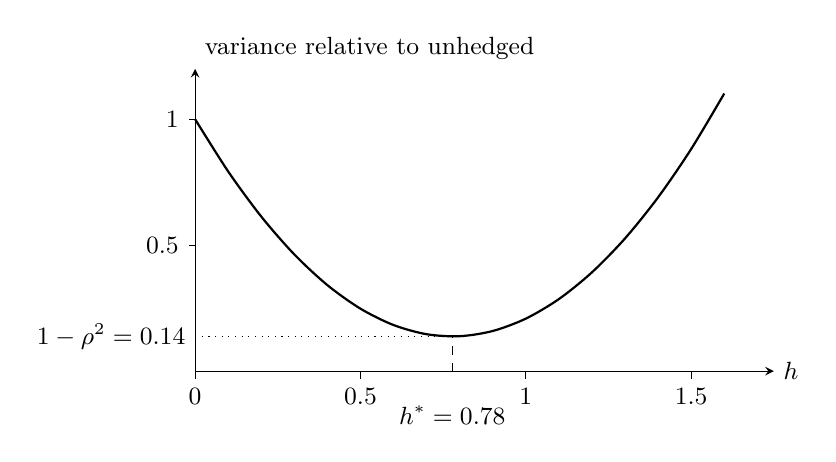
\begin{tikzpicture}[>=stealth, x=4.2cm, y=3.2cm, font=\small]
  \draw[->] (0,0) -- (1.75,0) node[right] {$h$};

  \draw[->] (0,0) -- (0,1.2) node[above right] {variance relative to unhedged};
  \foreach \x in {0,0.5,1,1.5} \draw (\x,0) -- (\x,-0.03) node[below] {\x};
  \foreach \y in {0.5,1} \draw (0,\y) -- (-0.02,\y) node[left] {\y};
  \draw[thick] plot[smooth] coordinates {(0.00,1.0000) (0.10,0.7926) (0.20,0.6137) (0.30,0.4633) (0.40,0.3414) (0.50,0.2480) (0.60,0.1831) (0.70,0.1467) (0.80,0.1388) (0.90,0.1595) (1.00,0.2086) (1.10,0.2862) (1.20,0.3924) (1.30,0.5270) (1.40,0.6901) (1.50,0.8818) (1.60,1.1019)};
  \draw[dashed] (0.7777,0) node[below=9pt] {$h^*=0.78$} -- (0.7777,0.1381);
  \draw[dotted] (0,0.1381) node[left] {$1-\rho^2=0.14$} -- (0.7777,0.1381);
\end{tikzpicture}

\caption{Variance of $\Delta S-h\Delta F$ relative to the unhedged variance for Hull's jet-fuel and heating-oil data (Table~3.2, p.~82), computed for this entry; the minimum is at $h^*$, as in Hull's schematic Figure~3.3 (p.~81).}\label{fig:hedge-variance}
\end{figure}

\qffield{Pitfalls} The legacy tailing rule ``$N^*/(1+0.01r)$'' holds only for one year remaining, as in Hull's example. The legacy ``standard deviation is minimised by setting $h=b$'' needs $\epsilon$ uncorrelated with $\Delta F$, which OLS guarantees in sample. Hull's index-hedge table assumes a predictable dividend yield, a constant risk-free rate and perfect correlation between portfolio and index returns, so ``in practice \dots\ the hedge works rather less well'' (p.~87, n.~5); CAPM supplies an expected return there, not a guarantee. Hull's reasons for index hedging (confidence in stock selection, short-term protection without selling) are motivations, not evidence that such hedges add value (pp.~87--88).

\qffield{See also} \hyperref[def:futures-hedge-basis]{futures hedges and basis}; \hyperref[mod:factor-risk-model]{factor risk model} (beta as a factor exposure); \hyperref[mod:duration-convexity]{duration and convexity}.

\qffield{Further reading} Time-varying and GARCH hedge ratios, and the evidence on hedging's value, are the pathway's readings (backlog). The legacy file and its original figure are kept verbatim in \nolinkurl{notes/artefacts/volatility-options/}.

\qffield{Index} hedge ratio; minimum-variance hedge ratio; optimal hedge ratio; hedge effectiveness; R-squared; correlation; regression slope; number of contracts; daily settlement; percentage changes; tailing the hedge; stock index futures; beta; changing beta; cross hedge

\qffield{Status} Verification: partly checked 2026-10-15 (against the text layer of a local copy of \texttt{s7-hulloptions}, 11th Global edition, chap.~3, pp.~79--90; Table~3.2 recomputed, the variance minimised numerically and the curve plotted; the derivation is the entry's own). Stability: draft. Currency: timeless; data as of Hull's example.
\end{qfmodel}
